% !TEX encoding = IsoLatin2  % notwendige Zeile für Mac-Benutzer (muss als Kommentar stehen); Windows-Benutzer können die Zeile löschen.

% LaTeX-Vorlage Version 3.1,  Juli 2011
% erstellt von Dr. Andreas Drauschke (andreas.drauschke@technikum-wien.at) und Dr. Susanne Teschl (susanne.teschl@technikum-wien.at)
% geringfügig adaptiert von Harald Stockinger (harald.stockinger@technikum-wien.at)

 
\documentclass[a4paper,bibtotoc,oneside]{scrbook} 
% Für kurze Arbeiten wäre auch die Dokumentklasse "scrartcl" ausreichend. In diesem Fall ist "section" die höchste Ebene ("chapter" gibt es dann nicht).
% \documentclass[a4paper,bibtotoc,oneside]{scrartcl}

%\usepackage{cclicenses}

% javascript highlightning support
\usepackage{listings}
\usepackage{color}
\definecolor{lightgray}{rgb}{.9,.9,.9}
\definecolor{darkgray}{rgb}{.4,.4,.4}
\definecolor{purple}{rgb}{0.65, 0.12, 0.82}

\lstdefinelanguage{JavaScript}{
  keywords={typeof, new, true, false, catch, function, return, null, catch, switch, var, if, in, while, do, else, case, break},
  keywordstyle=\color{blue}\bfseries,
  ndkeywords={class, export, boolean, throw, implements, import, this},
  ndkeywordstyle=\color{darkgray}\bfseries,
  identifierstyle=\color{black},
  sensitive=false,
  comment=[l]{//},
  morecomment=[s]{/*}{*/},
  commentstyle=\color{purple}\ttfamily,
  stringstyle=\color{red}\ttfamily,
  morestring=[b]',
  morestring=[b]"
}
\lstset{
   language=JavaScript,
   backgroundcolor=\color{lightgray},
   extendedchars=true,
   basicstyle=\footnotesize\ttfamily,
   showstringspaces=false,
   showspaces=false,
   numbers=left,
   numberstyle=\footnotesize,
   numbersep=9pt,
   tabsize=2,
   breaklines=true,
   showtabs=false,
   captionpos=b
}

% verlinkte Querverweise im pdf
\usepackage{hyperref}

% deutsche Anpassungen
\usepackage[utf8]{inputenc}
\usepackage[T1]{fontenc}
\usepackage[ngerman]{babel}


% mathematische Symbole
\usepackage{amsmath,amssymb,amsfonts,amstext}

% Kopfzeilen frei gestaltbar
\usepackage{fancyhdr}
\lfoot[\fancyplain{}{}]{\fancyplain{}{}}
\rfoot[\fancyplain{}{}]{\fancyplain{}{}}
\cfoot[\fancyplain{}{\footnotesize\thepage}]{\fancyplain{}{\footnotesize\thepage}}
\lhead[\fancyplain{}{\footnotesize\nouppercase\leftmark}]{\fancyplain{}{}}
\chead{}
\rhead[\fancyplain{}{}]{\fancyplain{}{\footnotesize\nouppercase\sc\leftmark}} 

% Farben im Dokument möglich
\usepackage{color}

% Schriftart Helvetica
\usepackage{helvet}
\renewcommand{\familydefault}{cmss} 

% Graphiken einbinden: hier für pdflatex
\usepackage[pdftex]{graphicx}

\usepackage{array}

% Höhe und Breite des Textkörpers etwas grösser definieren
\setlength{\textheight}{225mm}
\setlength{\textwidth}{1.05\textwidth}

% weniger Warnungen wegen überfüllter Boxen
\tolerance = 9999
\sloppy

% Anpassung einiger überschriften 
\renewcommand\figurename{Abbildung}
\renewcommand\tablename{Tabelle}

\begin{document}

% Kopf- und Fusszeilen initiieren
\pagestyle{fancy}
\pagenumbering{Alph}

% Deckblatt:
\thispagestyle{empty}
\begin{picture}(0,0)
\color{white}\sffamily
\put(-101,-749){
\includegraphics[width=1.002\paperwidth, height=\paperheight]{BM_2011.pdf}}
\put(220,-670){
\includegraphics[width=0.5\textwidth]{FHTW_Logo_4c.pdf}}
\put(-30, -20){\bfseries\huge BACHELORARBEIT}
% Titel des Studienganges einfügen:
\put(-30,-50){\Large im Studiengang Bachelor Informatik}
% Titel der Arbeit einfügen:
% Die Minipage wird gesetzt, damit auch mehrzeilige Titel möglich werden.
\put(-32,-150){
\begin{minipage}{14cm}
\bfseries\huge Software-Test von Web-Applikationen
\end{minipage}
}
% Name der Autorin/des Autors eingeben:
\put(-30,-250){\large Ausgeführt von: Bernhard Posselt}
% Personenkennzeichen der Autorin/des Autors eingeben:
\put(-30,-270){\large Personenkennzeichen: 1010257029}
% Name der Begutachterin/des Begutachters eingeben:
\put(-30,-310){\large Begutachter: Benedikt Salzbrunn, MSc}
\put(-30,-350){\large Wien, \today} % das Datum des letzten Kompilierens wird automatisch eingesetzt
\color{black}
\end{picture}

\newpage


\section*{Eidesstattliche Erklärung}\thispagestyle{empty}
\glqq Ich erkläre hiermit an Eides statt, dass ich die vorliegende Arbeit selbständig angefertigt habe. 
Die aus fremden Quellen direkt oder indirekt übernommenen Gedanken sind als solche kenntlich gemacht. 
Die Arbeit wurde bisher weder in gleicher noch in ähnlicher Form einer anderen Prüfungsbehörde vorgelegt
und auch noch nicht veröffentlicht. Ich versichere, dass die abgegebene Version jener im Uploadtool entspricht.\grqq\\[5\baselineskip]
\rule{5cm}{0.2pt}\hfill\rule{5cm}{0.2pt}\\
\phantom{Datum }Ort, Datum\hfill Unterschrift\hspace{15mm}

\newpage


\section*{Kurzfassung}\thispagestyle{empty}
Die Durchführung und Erstellung von automatisierten Tests für Web-Applikationen unterscheidet sich von klassischen Applikationen: Aufgrund der komplexeren Infrastruktur und Modularisierung werden zusätzliche Testfälle und Strategien benötigt um Web-Applikationen ausreichend abzudecken und eine fortwährende Qualität zu gewährleisten. Diese Arbeit soll Möglichkeiten für den Test von Web-Applikationen anhand eines Projektes aufzeigen und Anpassungen und Anwendung der vier Testformen des V-Modells: Unit Test, Integration Test, System Test und Acceptance Test. 

\vfill
\paragraph*{Schlagwörter:} Webapplikationen, automatisierte Tests, Webtest
% TODO: http://opus.bsz-bw.de/xgnd/index.php schlagwörter checken

\newpage

\section*{Abstract}\thispagestyle{empty}
Creation and execution of automatic web application tests is different from tests of classic applications. A more complex infrastructure and modularisation require additional testcases and strategies to guarantee a good enough test coverage which in return ensures constant quality. This thesis highlights various possibilities to test web applications based on a real world project and shows how to use and adjust the V-Model's four test methods: Unit Test, Integration Test, System Test and Acceptance Test.

\vfill
\paragraph*{Keywords:} web applications, automatic tests, webtest
\newpage

%\section*{Danksagung}
%\thispagestyle{empty}
%Text Text Text Text Text Text Text Text Text Text Text Text Text Text Text Text
%\newpage

\tableofcontents\thispagestyle{empty}
\newpage

\pagenumbering{arabic}
\setcounter{page}{1}

% Falls die Kapitelüberschriften zu lang für die Kopfzeile oder das Inhaltsverzeichnis sind, so erzielt man
% dort Kurzformen der Kapitelbezeichnungen mittels:
% \chapter[Kurzform]{Lange überschrift}
\chapter{Einführung}
Der Markt für elektronische Geräte hat in den letzten Jahren ein rasantes Wachstum erlebt, vor allem im Bereich der mobilen Geräte. Im Jahr 2011 wurden erstmals mehr mobile Geräte verkauft als PCs (Abbildung \ref{Abb1}).
Aufgrund des starken Wachstums dehnt sich der Markt für Software-Applikationen auch auf mobile Geräte aus, welche zum Großteil andere Betriebssysteme und Applikations-Frameworks verwenden als traditionelle Computer (Abbildung \ref{Abb2}). Viele dieser Plattformen erfordern das Erlernen von unterschiedlichen Programmiersprachen, Frameworks und Betriebssystemen \cite{android}\cite{ios}. Will ein/eine Software-EntwicklerIn eine Applikation plattformübergreifend anbieten, erfordert dies daher einen höheren Zeit- und Kostenaufwand.

\begin{figure}[h!]
\centering
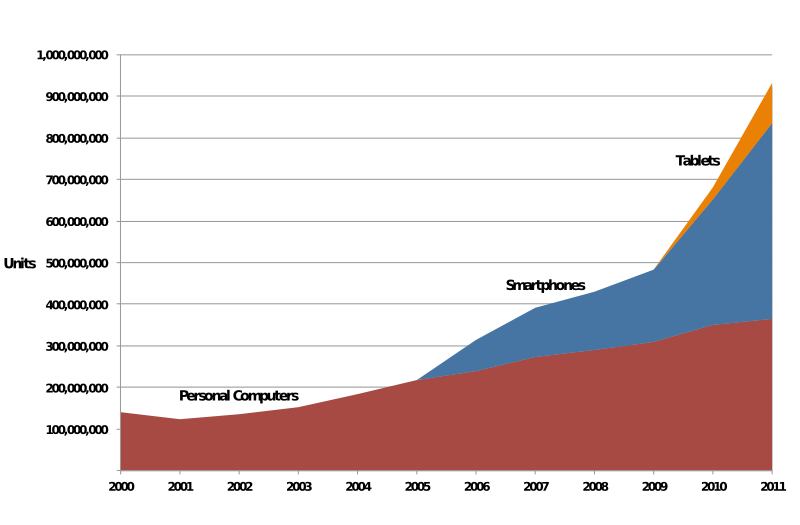
\includegraphics[width=150mm]{img/globaldevicesales.png}
\caption[Entwicklung der PC und Mobilgerätverkäufe]{Entwicklung der PC und Mobilgerätverkäufe \cite{devicesales}[S. 6]}\label{Abb1}
\end{figure}
% TODO: grafik verbessern, klarer machen
% TODO: formulieren, mehr plattformübergreifender, weniger mobilbereich

Da viele dieser Mobilgeräte über einen Web-Browser verfügen, wird das Web als Applikations-Plattform immer attraktiver. Zudem erlauben Frameworks wie PhoneGap \cite{phonegap} dem/der EntwicklerIn eine plattformübergreifende Mobil-Applikation auf Web-Technologie-Basis zu erstellen, welche sich nahtlos in das System integrieren. 

\begin{figure}[h!]
\centering
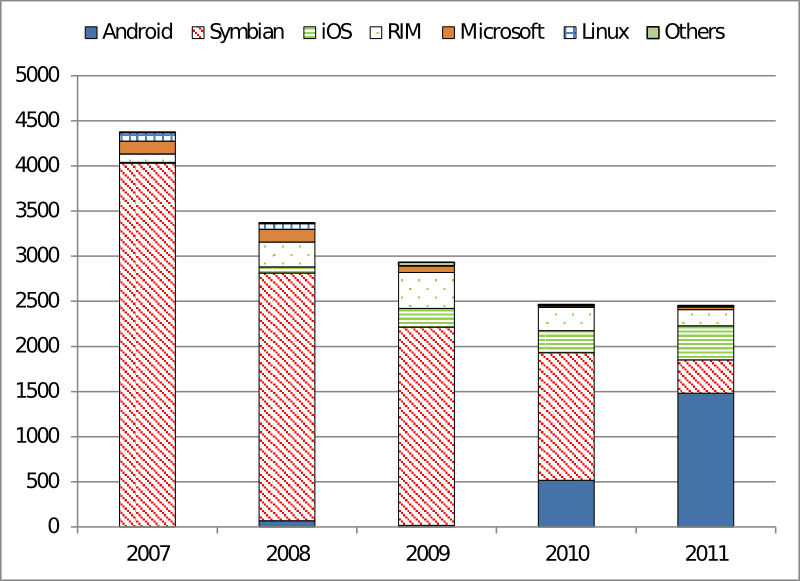
\includegraphics[width=130mm]{img/operatingsystems.png}
\caption[Marktanteil mobiler Betriebssysteme]{Marktanteil mobiler Betriebssysteme \cite{smartphone}[S. 22]}\label{Abb2}
\end{figure}
% TODO: legende

\section{Problemstellung}
Aufgrund der Vielfalt an unterschiedlichen Web-Browsern erhöht sich jedoch auch der Testaufwand der Applikation. Die Browser implementieren die vom W3C vorgeschlagenen Standards ab und zu anders und in unterschiedlicher Geschwindigkeit. Nicht selten kommt es vor, dass gewisse Funktionen nur in einer eingeschränkten Auswahl von Web-Browsern voll funktionsfähig sind und zusätzliche Anpassungen erfordern. \cite{caniuse}

Ein weiteres Problem ist das verhaltene Upgradeverhalten der NutzerInnen. Im Falle des Internet Explorers 7 dauerte es beispielsweise länger als 19 Monate, bis rund die Hälfte der NutzerInnen auf die neue Version umgestiegen sind. \cite{insecure}[S. 3]

All dies zwingt Web-EntwicklerInnen eine Vielzahl an unterschiedlichen Browsern und Browser-Versionen zu unterstützen.


\section{Lösungsansatz}
Um eine konstante Qualität der Web-Applikation auf allen Plattformen zu gewährleisten, muss das bisherige Testssystem angepasst werden, um der höheren Komplexität von Web-Applikationen gerecht zu werden. 

% Lösungsansatz: herausforderungen kein ansatz, überblick auch nicht, mehr auf beispiele eingehen
Diese Bachelorarbeit zeigt zusätzlichen Herausforderungen beim Testen von Web-Applikationen aufzeigen. Des Weiteren soll sie einen Überblick über mögliche Anwendungen und Anpassungen der vier häufigsten Testarten - den Unit Tests, Integration Tests, System Tests und Acceptance Tests - im Bereich der Web-Applikationen geben. Dazu wird anhand eines Projektes eine Test-Strategie erarbeitet und Beispiele für Tests gegeben.

\newpage

\section{Aufbau}
% nicht nur auf kapitel eingehen, sondern inhaltlich gruppieren
Kapitel 2 behandelt den Sinn und die Grenzen des Software-Tests und wie er sich in den Entwicklungsprozess einbinden lässt. Außerdem wird anhand des V-Modells versucht, den Zusammenhang zwischen Software-Test und Projektablauf aufzuzeigen.

In Kapitel 3 wird auf die Unterschiede zwischen klassischen Applikationen und Web-Applikationen eingegangen. Dadurch sollen zusätzliche Probleme, die sich durch das Applikations-Modell ergeben, aufgezeigt werden.

Die Planung und der Ablauf des Testprozesses durch die Verwendung eines Testplanes Kapitel 4 beschrieben. 

Kapitel 5 beschäftigt sich näher mit dem praktischen Einsatz von client- und serverseitigen Unit Tests. Es werden für beide Seiten Beispiele eines Unit Tests gezeigt und auf klassiche Probleme bei clientseitigen Unit Tests und deren Lösungen eingangen.

Das Thema des Integration Tests wird in Kaptitel 6 behandelt. Außerdem wird auf die verschiedenen Test-Ansätze eingegangen.

Kaptitel 7 behandelt den Systemtest. Es wird anhand von Beispielen gezeigt, wie die verschiedenen Server- und Client-Plattformen automatisch getestet werden können.

Kapitel 8 beschäftigt sich mit dem Thema des Acceptance Tests und wie dieser bei Web-Applikationen umgesetzt werden kann.

\chapter{Warum testen}
Keine Applikation ist fehlerfrei\cite{empiric_invest}[S. 9]. Diese Fehler  führen nicht nur zu unzufriedenen Kunden, sondern auch zu hohen Kosten: \glqq Im Jahr 2000 wurde in den USA ein Schaden durch Softwarefehler in der Auto- und Flugzeugindustrie von 1,8 Milliarden US-Dollar errechnet. Dies entspricht ca. 16 \% des Softwareumsatzes.\grqq\cite{betrieb}[S. 15]

Die Fehler-Rate wird auf ungefähr 3 pro 1.000 Zeilen geschätzt, was bei einer aufwendigeren Applikation mit 100 Millionen Zeilen Quellcode eine durchschnittliche Anzahl von 300.000 Fehlern ergibt \cite{eval_regression}[S. 10]. 

Je früher diese Fehler entdeckt werden, desto kostengünstiger können diese beseitigt werden \cite{betrieb}[S. 17]. Daher ist es wichtig, möglichst früh mit dem Testen zu beginnen und den Software-Entwicklungsprozess dementsprechend anzupassen \cite{betrieb}[S. 16]. 

\section{Verschiedene Testarten}
Laut dem V-Modell (Abbildung \ref{Abb3}) ist der Software-Test kein seperater Abschnitt im Projektplan. Vielmehr ist er ein Prozess, der die verschiedenen Entwicklungsabschnitte ergänzt \cite{betrieb}[S. 23]. Das V-Model unterscheidet zwischen vier verschiedenen Testarten:

\begin{itemize}
	\item Unit Test: Wird paralell zur Implementation erstellt
	\item Integration Test: Wird erstellt, um den Designprozess zu überprüfen
	\item System Test: Testet die konkreten Anforderungen an die Software
	\item Acceptance Test: Testet die Anforderungen des Kunden
\end{itemize}

\begin{figure}[h!]
\centering
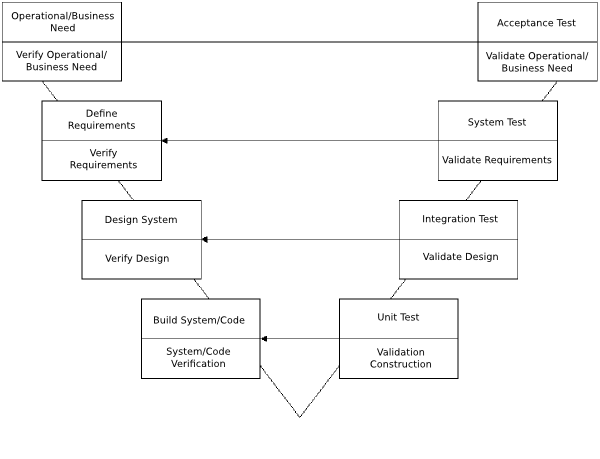
\includegraphics[width=120mm]{img/vmodel.png}
\caption[Schematische Darstellung des V-Modells]{Schematische Darstellung des V-Modells \cite{vmodel}[S. 3]}\label{Abb3}
\end{figure}

Tests können jedoch nicht nur dazu verwendet werden, um Fehler in der Applikation zu finden, sondern auch um einen Überblick über den derzeitigen Stand der Implementation zu gewinnen: Sie geben dem/der EntwicklerIn und ProjektmanagerIn ein direktes Feedback über bereits korrekt implementierte Teile der Software-Spezifikation. Auch Milestones können durch Tests definiert werden. \cite{test_auto}[S. 2]

Zudem ist eine Abschätzung riskanter Bereiche möglich, die durch eine erhöhten Testbedarf bestimmter Bereiche offensichtlich wird. \cite{testing_apps_on_web}[S. 34]


\section{Manuelle Tests}
Manuelle Tests eignen sich vor allem im Bereich des System Tests und Acceptance Tests, da sich diese Bereiche oft schwer komplett automatisch testen lassen. Darunter fallen z.B. Kontrollen der Übersetzungen und der Dokumentation, Usability Tests, externe Beta Tests, Security Tests und explorative Tests. \cite{test_large_systems}[S. 61]


\section{Automatisierte Tests}
Da die vorhandenen Tests durch die Einbindung in den Entwicklungsprozess öfters durchgeführt werden müssen, kann durch das repetetive Durchführen immergleicher Prozesse beim/bei der TesterIn schnell eine gewisse Eintönigkeit und Genervtheit entstehen. Das wiederum kann unter anderem dazu führen, dass TesterInnen im Laufe der Zeit bestimmte Tests nicht korrekt oder ineffizient ausführen. 

Die Lösung des Problems ist die teilweise Automatisierung des Testprozesses. Diese erlaubt bei zukünftigen Testdurchläufen nicht nur eine starke Reduzierung des Zeitaufwandes pro Durchlauf, sondern ermöglicht es auch, die Tests rund um die Uhr durchzuführen. Oft werden am Abend alle zeitintensiven Tests gestartet, damit die EntwicklerInnen am nächsten Morgen einen guten Überblick darüber haben, was nicht oder nicht mehr funktioniert. \cite{test_auto}[S. 22-23]

Es gibt mehrere Faktoren, die bei der Entscheidung der Automatisierung berücksichtigt werden müssen. 

% TODO: klarer trennen, absätze checken, bulletpoints?

Erstens muss klar sein, dass der Aufwand der Testerstellung einen wirtschaftlichen Nutzen hat. Bei einer sehr kleinen und unkritischen Applikation kann es sich z.B. nicht lohnen, Tests zu automatisieren. Dies liegt unter anderem daran, dass Tests erst über einen längeren Zeitraum ihre volle Stärke ausspielen. \cite{eval_regression}[S. 12]

Zweitens muss das Personal über eine dementsprechende Ausbildung verfügen, die Tests zu automatisieren. \cite{eval_automat_webapp_test}[S. 37]

Drittens eignet sich nicht jede Testart zur vollkommenen Automatisierung. Währen Unit-Tests und Integration-Tests sehr gut automatisiert werden können, ist es schon schwieriger System- und Acceptance Tests zu automatisieren. 

\section{Grenzen von Software-Tests}
Software-Tests können nie eine komplett fehlerfreie Software garantieren. Es kann höchstens eine Fehlerabwesenheit für jene Fälle garantiert werden, welche mit Tests abgedeckt wurden. \cite{eval_regression}[S. 12]. 

Dies resultiert unter anderem daraus, dass die Anforderungen an die Software oft nicht komplett spezifiziert oder zu ungenau formuliert sind. Zusätzlich steigt die Komplexität der Applikation im Laufe der Entwicklung stark an. Ein weiterer Grund stellt die oft schier unbegrenzten Möglichkeiten an unterschiedlichen Eingaben dar. \cite{software_qual}[S. 243].

Die implementierten Testfälle müssen auch regelmäßig gewartet und aktualisiert werden, um ihre Effektivität zu gewährleisten, denn diese nimmt auf Dauer ab. Es ensteht eine sogenannte \glqq Testresistenz\grqq\cite{eval_regression}[S. 12], die daraus resultiert, dass die bestehenden Tests nur bekannte Fehlerfälle abdecken und keine neuen, mögliche Fehlerfälle berücksichtigen. \cite{eval_regression}[S. 12-13]

\chapter{Testplan}

Mit dem Erstellen des Projektplanes sollte gleichzeitig auch ein Testplan erstellt werden \cite{eval_automat_webapp_test}[S. 24]. Dieser erlaubt, den Testprozess näher zu spezifizieren und somit den erforderlichen Aufwand besser abschätzbar zu machen \cite{test_large_systems}[S. 18]. Sollte es notwendig sein, kann damit der Testprozess auch an ein externes Team ausgelagert werden. Wird der Testplan zudem in den Abnahmenkriterien verankert, reduziert sich das Projektrisiko durch klar definierte Kriterien. \cite{eval_automat_webapp_test}[S. 26]

\section{Inhalt}
Im Testplan werden unter anderem folgende Punkte behandelt \cite{test_auto}[S. 3]:

\begin{itemize}
	\item Was wird getestet? Welche Bereiche besitzen eine höhere Priorität als andere?
	\item Wo wird getestet? Mit welchen Konfigurationen, Soft- und Hardware Plattformen respektive Versionen werden getestet?
	\item Wie wird getestet? mit welchen Tools wird getestet?
	\item Wer testet?
	\item Wie lange wird getestet? Bis wann muss ein Test erfolgreich absolviert werden?
	\item Was wird nicht getestet?
\end{itemize}


\section{Ablauf}
Da die Entwicklung der Applikation meistens unter einem hohen Zeitdruck abläuft\cite{software_qual}[S. 244] und der Testprozess zudem teuer ist \cite{eval_regression}[S. 24], ist es wichtig, Testfälle heraus zu arbeiten, zu priorisieren und effektiv zu verteilen. Auch Endkriterien sollten für die Tests veranschlagt und eine optimale Teststrategie gewählt werden.

Danach folgt die Überprüfung des Testplans. Hier wird überprüft, ob die einzelnen Testfälle genau genug beschrieben worden sind, um daraus die jeweiligen Testfälle erstellen zu können. Auch die Effiktivität der Teststrategien wird überprüft. Diese Prüfung findet nicht nur einmal statt, sondern wiederholt sich mehrfach im Testprozess. Dies hängt damit zusammen, dass die Anforderungen an die Software im Laufe der Implementation immer konkreter werden und somit auch neue, mögliche Fehlerfälle enstehen können.\cite{eval_regression}[S. 25] 

Ist der Testplan soweit fertig, kann ein Zeitplan für die einzelnen Testfälle erstellt werden. In weiterer Folge werden die einzelnen Tests an die TesterInnen vergeben. Diese können nun mit der Erstellung der konkreten Testfälle beginnen können.

Manche Tests haben eine sehr hohe Laufzeit. Um den Ablauf daher zu beschleunigen, wird ein Smoke-Tests erstellt. Der Smoke-Test testet grobe Szenarien der Applikation. Schlagen diese fehl, sind weitere Testdurchläufe nicht notwendig und der Testdurchlauf kann abgebrochen werden. 

Nach dem Ausführen der Tests wird ein Bericht erstellt. Je nach Ausgang der Tests muss der Testplan angepasst werden. Verliefen alle Tests positiv, kann das die jeweilige Phase abgeschlossen werden. \cite{eval_regression}[S. 26]


\section{Vorteile eines Testplans}

Aufgrund der Dokumentation der Testfälle, ergeben sich zusätzlich folgende Vorteile:

\begin{itemize}
	\item Fehlende Testfälle können schnell erkannt werden \cite{test_large_systems}[S. 18]
	\item Redundante Testfälle werden identifziert, Testfälle können zusammegelegt werden um Zeit zu sparen \cite{testing_apps_on_web}[S. 34]
	\item Verschiedene Testbereiche können an mehrere Personen mit unterschiedlichen Fachkenntnissen verteilt werden um Personalengpässe zu vermeiden \cite{test_large_systems}[S. 19]
	\item Ineffiziente Test-Tools und Test-Strategien können erkannt und verbessert werden \cite{eval_regression}[S. 25]
	\item Geschäftskritische Bereiche und solche mit einer erhöhten  Fehleranfälligkeit werden sichtbarer \cite{testing_apps_on_web}[S. 34]. Dies ist vor allem wichtig, da Fehler ungleich verteilt sind und in bestimmten Bereichen häufiger vorkommen als in anderen \cite{eval_regression}[S. 12]
	\item Sinnlose Testfälle und Testbereiche können aussortiert werden 
	\item Abhängigkeiten der Testfälle untereinander und der Implementation werden transparent und erlauben schnell auf Änderungen zu reagieren\cite{test_auto}[S. 4]
\end{itemize}

% geht um unterschiede im tests, unterschieden von klassischer noch nicht da
\chapter{Unterschiede zu klassischer Software}
Eine Web-Applikationen unterscheidet sich an mehreren Stellen von einer klassichen Applikation, was das Testen und das Auffinden von Fehlern zusätzlich erschwert. Die Hauptunterschiede sind:

\begin{itemize}
	\item Modularer Aufbau
	\item Plattformunabhängigkeit
	\item Session Modell
\end{itemize}


\section{Modularer Aufbau}

Im Gegensatz zu klassischen Desktop- oder Mobil-Applikationen bestehen Web-Applikationen wegen ihrer Client-Server-Architektur immer aus mehreren Modulen (Abbildung \ref{Abb4}). Diese Module sind meist über ein Netzwerk miteinander verbunden.

Durch diesen modularen Aufbau ist es besonders schwer einen Fehler zu lokalisieren. Ein Fehler kann z.B. durch einen Fehler im Quellcode des Applikations-Servers oder durch ein Netzwerkproblem entstanden sein. \cite{testing_apps_on_web}[Foreword]

\begin{figure}[h!]
\centering
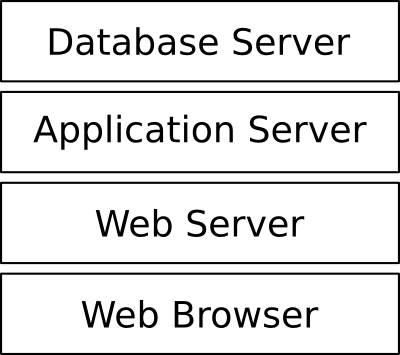
\includegraphics[width=50mm]{img/webstack.png}
\caption[Typischer Aufbau einer Web-Applikation]{Typischer Aufbau einer Web-Applikation}\label{Abb4}
\end{figure}

\section{Unterstützung mehrerer Plattformen}
Web-Applikationen laufen auf einer Vielzahl verschiedener Plattformen, Server- und Clientseitig. Dies ermöglicht dem/der EntwicklerIn Zeit und Aufwand zu sparen, befreit ihn/sie jedoch nicht von der Aufgabe, sicher zu stellen, dass die Applikation auf möglichst vielen Plattformen korrekt ausgeführt wird.

Während auf der Serverseite die jeweilig zu verwendenden Plattformen noch vom/von der BetreiberIn festlegbar sind, sprich welches Betriebssystem und welche Datenbank eingesetzt wird, ist dies auf der Clientseite schon nicht mehr möglich. 

Die BesucherInnen der Webseite verwenden unterschiedliche Web-Browser auf verschiedenen Betriebssystemen in unterschiedlichen Versionen. Auch können unterschiedliche Plugins und Fonts in unterschiedlichen Versionen installiert sein \cite{testing_apps_on_web}[Foreword]. Dies erhöht den Testaufwand, da bestimmte Funktionen nicht vorhanden sein bzw. anders funktionieren können \cite{caniuse}.

Eine weitere Herausforderung von clientseitigem Code stellt die asynchrone und eventbasierte Programmierung dar. Dies erschwehrt nicht nur die Erstellung von Testfällen sondern erhöht auch die möglichen Kombinationen, in der die Events eintreten können. Die Möglichkeit, dass durch eine Aktion, z.B. ein Mausklick auf einen Link, mehrere Events ausgelöst werden können erhöht die Komplexität noch weiter. \cite{testing_apps_on_web}[S. 18]

All diese Probleme werden durch eine zunehmende Verlagerung der Applikations-Logik von der Server- auf die Clientseite\cite{testing_apps_on_web}[S. 13] noch weiter verstärkt. 

\section{Session Modell}
Eine weitere Herausforderung stellt das Session Modell von Web-Applikationen dar: viele Web-Applikationen verwenden nur eine Session pro NutzerIn, erlauben aber mehrere gleichzeitige Logins. Werden mehrere Instanzen der Applikation gestartet - z.B. loggt sich der/die NutzerIn auf dem Mobiltelefon und dem Laptop auf der Webseite ein - kann dies zu Synchronisationsproblemen zwischen den einzelnen Instanzen führen: Wird in einer Instanz ein Eintrag gelöscht, kann dieser durch eine fehlerhafte Synchronisation in einer andere Instanz immer noch existieren und in weiterer Folge zu Fehlern führen. \cite{testing_apps_on_web}[S. 20]


Diese Vielfalt an verschiedenen möglichen Konfigurationen und Herausforderungen erfordert eine neue Herangehensweise an das Thema Software-Test: Die bestehenden Techniken sind \glqq zwar auch notwendig, aber nicht ausreichend, um die Qualität der Applikation sicherzustellen\grqq\ \cite{eval_automat_webapp_test}[S. 18]


\chapter{Projektumfeld}
TBD
% welche umgebung, systemlandschaft, testlandschaft
% TODO: warum spannend, aufbau des projektes

\chapter{Unit Test}
%TODO: mocks erklären, kleines code beispiel

Unit Tests werden verwendet, um Klassen, Module oder einzelne Komponenten zu testen. Sie sind Whitebox Tests, sprich die Implementationsdetails sind bekannt\cite{betrieb}[S. 26], und werden üblicherweise vom ProgrammiererInnen selbst erstellt. 

Zu den Vorteilen von Unit Tests zählen:

\begin{itemize}
	\item Gute Paralellisierbarkeit
	\item Sehr schnell ausführbar
	\item Früh einsetzbar
	\item Erlaubt die Aufteilung in kleine Teilprobleme
	\item Zeigt schwer zu verwendende Interfaces auf
\end{itemize}

% TODO: nachteile gleich formatieren, an den schluss versetzen mit zusammenfassung

Viele dieser Vorteile werden durch den Einsatz von Mocks erreicht, die die konkreten Implementationen ersetzen.

Nur Unit Tests alleine reichen jedoch nicht aus, um das Projekt komplett abzudecken, da sie keine Kommunikation zwischen den einzelnen Komponenten testen. Auch Tests für verschiedene Datenbanken können dadurch nicht abgedeckt werden. \cite{test_large_systems}[S. 52]\cite{betrieb}[S. 28]

\section{Serverseitige Unit Tests}
% TODO: auch DI und IOC und trennung von Logik/Darstellung
Serverseitige Unit Tests unterscheiden sich nicht nur anhand des eingesetzten Test-Frameworks, sondern auch anhand der gewählten Programmiersprache. 

In dieser Arbeit wird das Test-Framework PHPUnit eingesetzt. Ein konkreter Unit Test könnte so aussehen:

\lstinputlisting[language=java]{src/phpunit.php}
\lstinputlisting[language=java]{src/phpunittest.php}


\section{Clientseitige Unit Tests}
Im Gegensatz zum serverseitigen Code gibt es auf der Clientseite nur eine mögliche Programmiersprache, um Logik plattformübergreifend zu implementieren: \emph{JavaScript}. Für JavaScript gibt es mehrere Test-Frameworks, unter anderem Jasmine \cite{jasmine}, QUnit \cite{qunit} und Mocha \cite{mocha}.
In dieser Arbeit wird für die Implementation der clienseitigen Unit Tests Jasmine eingesetzt.

\subsection{Häufige Probleme bei clientseitigem Code}
Das Web ist noch recht jung und entwickelt sich rasant. Wurde es früher nur für Webseiten eingesetzt, sollen nun auf einmal komplette Applikationen entstehen. Dies überfordert viele Entwickler und resultiert oft in halbgaren Architekturen und schlampigen Umsetzungen. 

\subsubsection{Fehlende Trennung von Logik und Präsentation}
Die mit Abstand am beliebtesten Clientseitige JavaScript Library ist jQuery. Im Jahr 2011 verwendeten laut Alexa 45\% der Top 100.000 Webseiten eine JavaScript Library. Von diesen 45\% entfielen 63\% auf jQuery. \cite{jquery}[S. 107-108]

jQuery ist sehr einfach zu verwenden \cite{jquery}[S. 110], verleitet jedoch den/die ProgrammierIn aufgrund der Funktionsweise dazu, Präsentation und Logik stark miteinander zu verweben. Dies liegt unter anderem daran, dass die meisten jQuery-Methoden einen Selektor als ersten Parameter erwartet. Dieser Selektor funktioniert ähnlich wie ein CSS Selector und selektiert bestimmte Element im DOM. \cite{jquery_selectors}

Folgender Code soll dieses Problem verdeutlichen: Der angeführte Code führt einen AJAX Request aus und gibt abhängig von der zurückgegebenen Datenstruktur einen unterschiedlichen Text aus:

\lstinputlisting[language=Html]{src/jquery.html}
\lstinputlisting[language=JavaScript]{src/jquery.js}

Durch das verwenden des Selektors \emph{\#field .info span} ist der JavaScript Code nun abhänig von der HTML Struktur der Webseite. Verändert ein Designer  die Struktur des HTML-Codes, beispielsweise um die Ausgabe an einen anderen Ort zu verschieben, besteht die Gefahr, dass der Selektor nicht mehr die gewollten Elemente selektiert und damit der JavaScript-Code nicht mehr funktioniert.

\subsubsection{Verwendung von Globalen Objekten und Variablen}
JavaScript macht es einfach, globale Variablen zu verwenden: Es unterstützt nicht nur implizite \emph{Globals}\cite{js_patterns}[S. 11], sondern regelt den Zugriff auf das DOM über das globale \emph{window} Objekt\cite{js_patterns}[S. 13].

Dadurch werden ProgrammiererInnen dazu verleitet, globale Variablen und Objekte zu benutzen. Das wiederum erschwert die die Testbarkeit, da eine implizite Abhängigkeit ensteht, die für den Tester nicht sofort offensichtlich ist. Auch wird es schwieriger, den Code in Isolation zu testen.

\subsection{Lösungsansatz}
Die vorher aufgezeigten Probleme können mit Hilfe folgende Techniken gelöst werden:

\begin{itemize}
	\item Trennung der Logik und Präsentation durch Templates
	\item Vermeidung von globalen Objekten und Variablen
	\item Verwendung der Software-Patterns Dependency Injection und Inversion of Control, um Abhängigkeiten von Objekten und Funktionen offensichtlich und konfigurierbar zu machen
\end{itemize}

Um dies zu erreichen wird das JavaScript Framework \emph{AngularJS}\cite{angular} eingesetzt.

\subsubsection{Trennung von Logik und Präsentation}
AngularJS erlaubt das Erstellen eigener HTML-Attribute und HTML-Elemente. Diese werden \emph{Directives} genannt und werden für die Darstellungslogik verwendet.

Mit AngularJS würde das vorige jQuery Beispiel in etwa so aussehen:

\lstinputlisting[language=Html]{src/angular.html}
\lstinputlisting[language=JavaScript]{src/angular.js}

Das \emph{Scope} dient als Schnittstelle zwischen der Logik und der Präsentation und erlaubt einen bidirektionalen Datenaustausch. Beide Layer sind nun sauber voneinander getrennt: Der JavaScript Code referenziert keine DOM-Elemente mehr und so kann so isoliert getestet werden. Außerdem ist es nicht mehr möglich, durch bloßes Verschieben des HTML-Codes Fehler in der JavaScript Logik auszulösen.


\subsubsection{Injecten von Globalen Objekten und Variablen}
AngularJS bietet zudem einen Inversion of Control Container um dynamisch Abhängigkeiten unter den Objekten und Funktionen aufzulösen. Häufig benutzte globale Objekte werden schon fertig konfiguriert mitgeliefert: das \emph{window} Objekt etwa kann durch den Service \emph{\$window} injected werden. Dadurch können die Abhängigkeiten einfach in den Tests durch Mocks ausgetauscht werden.

\subsubsection{Unit Test}
Für das oben aufgeführte Beispiel kann nun ein dazugehöriger Unit Test erstellt werden.

Für den AJAX Request wird das \emph{\_\$httpBackend\_} Mock injected. Dies erlaubt den asynchronen Request in einen synchronen umzuwandeln. Auch ein neues Scope wird erstellt, um das korrekte Binding zwischen Präsentation und Logik testen zu können.

\newpage 

\lstinputlisting[language=JavaScript]{src/angularunit.js}



\chapter{Integration Test}
Integration Tests werden verwendet, um die Kommunikation zwischen einzelnen Klassen, Modulen und Komponenten und den Programm-Fluss zu testen. Sie funktionieren ähnlich wie Unit Tests, verwenden jedoch je nach Implementations-Strategie wenig bis keine Mocks und testen weniger Implementationsdetails. \cite{test_large_systems}[S. 53-54]

Auf ein Integration Test Beispiel wird deshalb verzichtet. %verharmlosen, ned dazupacken, keine neuen Codebeispiele

% TODO: auch vorteile + nachteile

Durch die vielen möglichen Kombinationen der einzelnen Module gibt es keine allgemein gültige Implementations-Strategie \cite{betrieb}[S. 29]. Die zwei häufigsten verwendeten Methoden zur Erstellung der Testfälle sind:

\begin{itemize}
	\item Nicht Inkrementelle Testfallerstellung
	\item Inkrementelle Testfallerstellung
\end{itemize}

\section{Nicht Inkrementelle Testfallerstellung}
Wird die nicht inkrementelle Testfallerstellung genutzt, werden die nicht vorhandenen Module mit Mocks ersetzt. Diese werden am Schluss dann durch die aktuelle Implementation ausgetauscht.

Dies mag vor allem am Anfang sehr aufwendig erscheinen, erlaubt jedoch schon früh die Kommunikation zwischen den einzelnen Bereichen zu testen. Auf diese Weise kann sehr schnell ein Überblick über den Implementationsstand der Software erlangt werden. Diese Methode eignet sich daher besonders für Agile Software-Entwicklung. \cite{test_large_systems}[S. 54-59] 

\section{Inkrementelle Testfallerstellung}
Bei der inkrementellen Testfallerstellung werden wenig bis gar keine Mocks erstellt. Stattdessen wird immer versucht, auf den bisherig erstellten Modulen aufzubauen. Dadurch werden die zuerst erstellten Module am Besten getestet.\cite{test_large_systems}[S. 54-59]
% TODO: verschiedene arten aufzeigen und eventuell verweisen
Dies eignet sich vor allem dann, wenn es bestimmte Module mit einer hohen Komplexität und Fehlerdichte gibt und das Erstellen von Mocks sehr schwer und aufwendig ist. \cite{test_large_systems}[S. 59]


% TODO: einzelne absätze stärken, aufzähl
\chapter{System Test}
TBD
% testet das gesamtsystem 
% funktionale und nicht funktionale tests aber eher nicht funktionale \cite{test_large_systems}[S. 60]
% auf installationsumgebung getestet
% oft schwierig weil es auf produktivsystem des kunden läuft
% testet abläufe auf unterschiedlichen betriebssystemen + configs
% installation
% security
% 
%\cite{betrieb}[S. 30-31]

% manueller test möglich, die dokumentation kann auch damit durchgetestet werden
%
%\cite{test_large_systems}[S. 60]


% todo: gherkin + chef beispiele

\chapter{Acceptance Test}
TBD
% TODO: verheiraten mit system test? erklären warum

% test von kunden auf vertragliche richtlinien, oft stark kunde miteinbezogen
% benutzbarkeit

%\cite{eval_regression}[S. 28]
%
%\cite{test_auto}[S. 11]
%
%Development acceptance tests:
% data driven \cite{test_auto}[S. 24]
% * Release acceptance tests (smoke tests): mainstream data + mainstream funktionen \cite{testing_apps_on_web}[S. 36]
% * Functional acceptance simple test: each dev release to test accessibility of key features on minimum configuration, no full functionality test (file saving example) \cite{testing_apps_on_web}[S. 37-38]

%Deployment acceptance tests:
%Full installation + configurations
% * Task-Oriented Functional Test: Features test (gherkin) against requirements, specs + design docs \cite{testing_apps_on_web}[S. 42]
% * Forced Error Test: testing for failures 
% * boundary test: test extreme inputs
% * system level test: test whole application \cite{testing_apps_on_web}[S. 43]
% * real world user level test: echte leute testen um fehler zu finden die man sonst übersieht
% * exploratory test: überlegen wo es probleme geben könnte und dort testen
% * stress test: limited resource conditions (memory, diskspace, network bandwidth)
% * Performance tests: testen wieviel das system verträgt
% * Regression tests: für bugs die schonmal aufgetreten sind \cite{testing_apps_on_web}[S. 44]
% * Compability + config tests: testen auf unterschiedlichen platformen
% * documentation test: testen von zb shortcuts \cite{testing_apps_on_web}[S. 45]
% * install uninstall test
% * UX tests
% * External beta tests \cite{testing_apps_on_web}[S. 46]
% * Secuirty tests
% * Unit tests
%\cite{test_large_systems}[S. 10]

%test ist mehr als simples aufnehmen und abspielen von inputs: ist redundant und eintönig, muss automatisiert werden muss geplant werden und auch generisch sein ansonsten braucht wartung der test skripte mehr aufwand und reibereien mit kollegen wenn sie etwas ändern
%automatisiertes monkey testing findet nur absturz bugs aber keine funktionalen bugs 


\chapter{Zusammenfassung}
TBD
% \cite{process_oop}[S. 30]

% TODO: Vergleich zu klassischen apps nochmal erläutern, vor + nachteile vllt auch tabellarisch, abkürzungsverzeichnis weglassen bei nur 2 abkürzungen, mehr abbildungen


%\\[2\baselineskip]
%Hier wird auf Abbildung~\ref{Abb1} verwiesen. 
%\begin{figure}[htbp]
%\centering
%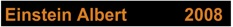
\includegraphics[width=75mm]{Buchruecken}
%\caption[Beschriftung eines Buchrückens.]{Beispiel für die Beschriftung eines
%Buchrückens.}\label{Abb1}
%\end{figure}
%%Tabelle~\ref{Tab1} ist ein Beispiel dafür, wie eine Tabelle aussehen könnte.
%\begin{table}[htbp]
%\centering
%\begin{tabular}{ | c | c | c | }\hline
%{\bf Datum} & {\bf Thema} & {\bf Raum}\\ \hline
%\hline
%20. 08. 2008 & Graphentheorie & HS 3.13\\ \hline
%01. 10. 2008 & Biomathematik & HS 1.05\\ \hline
%\end{tabular}
%\caption[Semesterplan "`Angewandte Mathematik"'.]{Beispiel für einen
%Semesterplan "`Angewandte Mathematik"'.}\label{Tab1}
%\end{table}

%\noindent
%Nun ein Beispiel für eine abgesetzte Formel:
%\begin{equation}
%x =  - \frac{p}{2} \pm \sqrt{\left(\frac{p}{2}\right)^2 - q}.
%\end{equation}
%Und eine mehrzeilige Formel:
%\begin{eqnarray}
%f(t)&=& t^2 \label{For1},\\
%g(t) &=& t-1.
%\end{eqnarray}
%Hier wird auf die Formel (\ref{For1}) verwiesen. \\

%\noindent
%So kann zum Beispiel ein \glqq Source-Code\grqq\  angegeben werden: 
%\begin{verbatim}
%for (i=1; i < 10; i++) {...} 
%\end{verbatim}

%\noindent
%Hier ist ein Hyperlink auf die  \href{http://www.technikum-wien.at}{Homepage}
%der FH Technikum Wien. Email-Adressen können so verlinkt werden:
%\href{mailto:homer.simpson@springfield.com}{\texttt{
%homer.simpson@springfield.com}}\\

%\noindent
%In der Bibliothek der Fachhochschule Technikum Wien gibt es verschiedene
%einführende Bücher zum Thema \glqq \LaTeX \grqq, zum Beispiel \cite{kop05},
%\cite{wil06} oder \cite{mgb+05d} (deutsche Version) bzw. \cite{mgb+04e}
%(englische Version). Empfehlenswerte Skripten für \LaTeX-Einsteiger sind z.B.
%\cite{mj00} und \cite{mj95}. Sie sind frei im Internet verfügbar.



% Literaturverzeichnis
% Das Literaturverzeichnis kann auch nach einem allfälligen Anhang positiioniert werden (siehe "`Leitfaden für Bachelor- und Diplomarbeiten"', Version 2.0, Abschnitt 2.9).

% Möglichkeit 1: Erzeugung des Literaturverzeichnisses mit BibTeX:
% Die Quellen sind in der Datei *.bib (hier Literatur.bib) einzugeben. Danach muss diese Vorlage einmal geTeXt werden, dann BibTeX angewendet werden und 
% anschliessend nochmals zweimal geTeXt werden.
% Im Text erfolgt die Zitierung mit dem Anker-Schlüsselwort, z.B. \cite{kop05}.
\bibliographystyle{IEEEtran}
\bibliography{Literatur}

% Möglichkeit 2: Erzeugung eines Literaturverzeichnisses ohne BibTeX:
%\begin{thebibliography}{99}
%\bibitem[kop05]{kop05}
%H.~Kopka, {\em LaTeX, Band 1: Einführung}, Pearson Studium, München, 3.~Auflage, 2005.
%\bibitem[knu98]{knu98}
%F.~Mittelbach, M.~Goossens, J.~Braams, D.~Carlisle, and Ch. Rowley, {\em The LaTeX Companion}, 
%Addison-Wesley, 2nd edition, 2004.
%\end{thebibliography}

% Abbildungsverzeichnis
\listoffigures
\addcontentsline{toc}{chapter}{Abbildungsverzeichnis} % fügt den Eintrag äbbildungsverzeichnis" im Inhaltsverzeichnis hinzu
\newpage

% Tabellenverzeichnis
%\listoftables 
%\addcontentsline{toc}{chapter}{Tabellenverzeichnis} % fügt den Eintrag
%"Tabellenverzeichnis" im Inhaltsverzeichnis hinzu
%\newpage

% Abkürzungsverzeichnis
% Bei Verwendung der Dokumentklasse "scrartcl" ist der Befehlt \addchap{Abkürzungsverzeichnis} durch 
% \addsec{Abkürzungsverzeichnis} zu ersetzen
\addchap{Abkürzungsverzeichnis}
\hspace{-17mm}\begin{tabular}{>{\raggedleft}p{0.2\linewidth} p{0.75\linewidth} p{0.1\linewidth}}

www & World Wide Web\\
CSS & Cascading Style Sheets\\
AJAX & Asynchron JavaScript And XML\\
HTML & HyperText Markup Language\\
DOM & Document Object Model\\
W3C & World Wide Web Consortium\\

\end{tabular}

% Anhänge
%\begin{appendix}
%\chapter[Erster Anhang]{überschrift des ersten Anhangs}

%Text Text Text Text Text Text Text Text Text Text Text Text Text Text Text Text
%\end{appendix}

\end{document}
